\chapter{Supplemental information for Chapter 3}


\begin{figure}
    \centering
    \makebox[\textwidth][c]{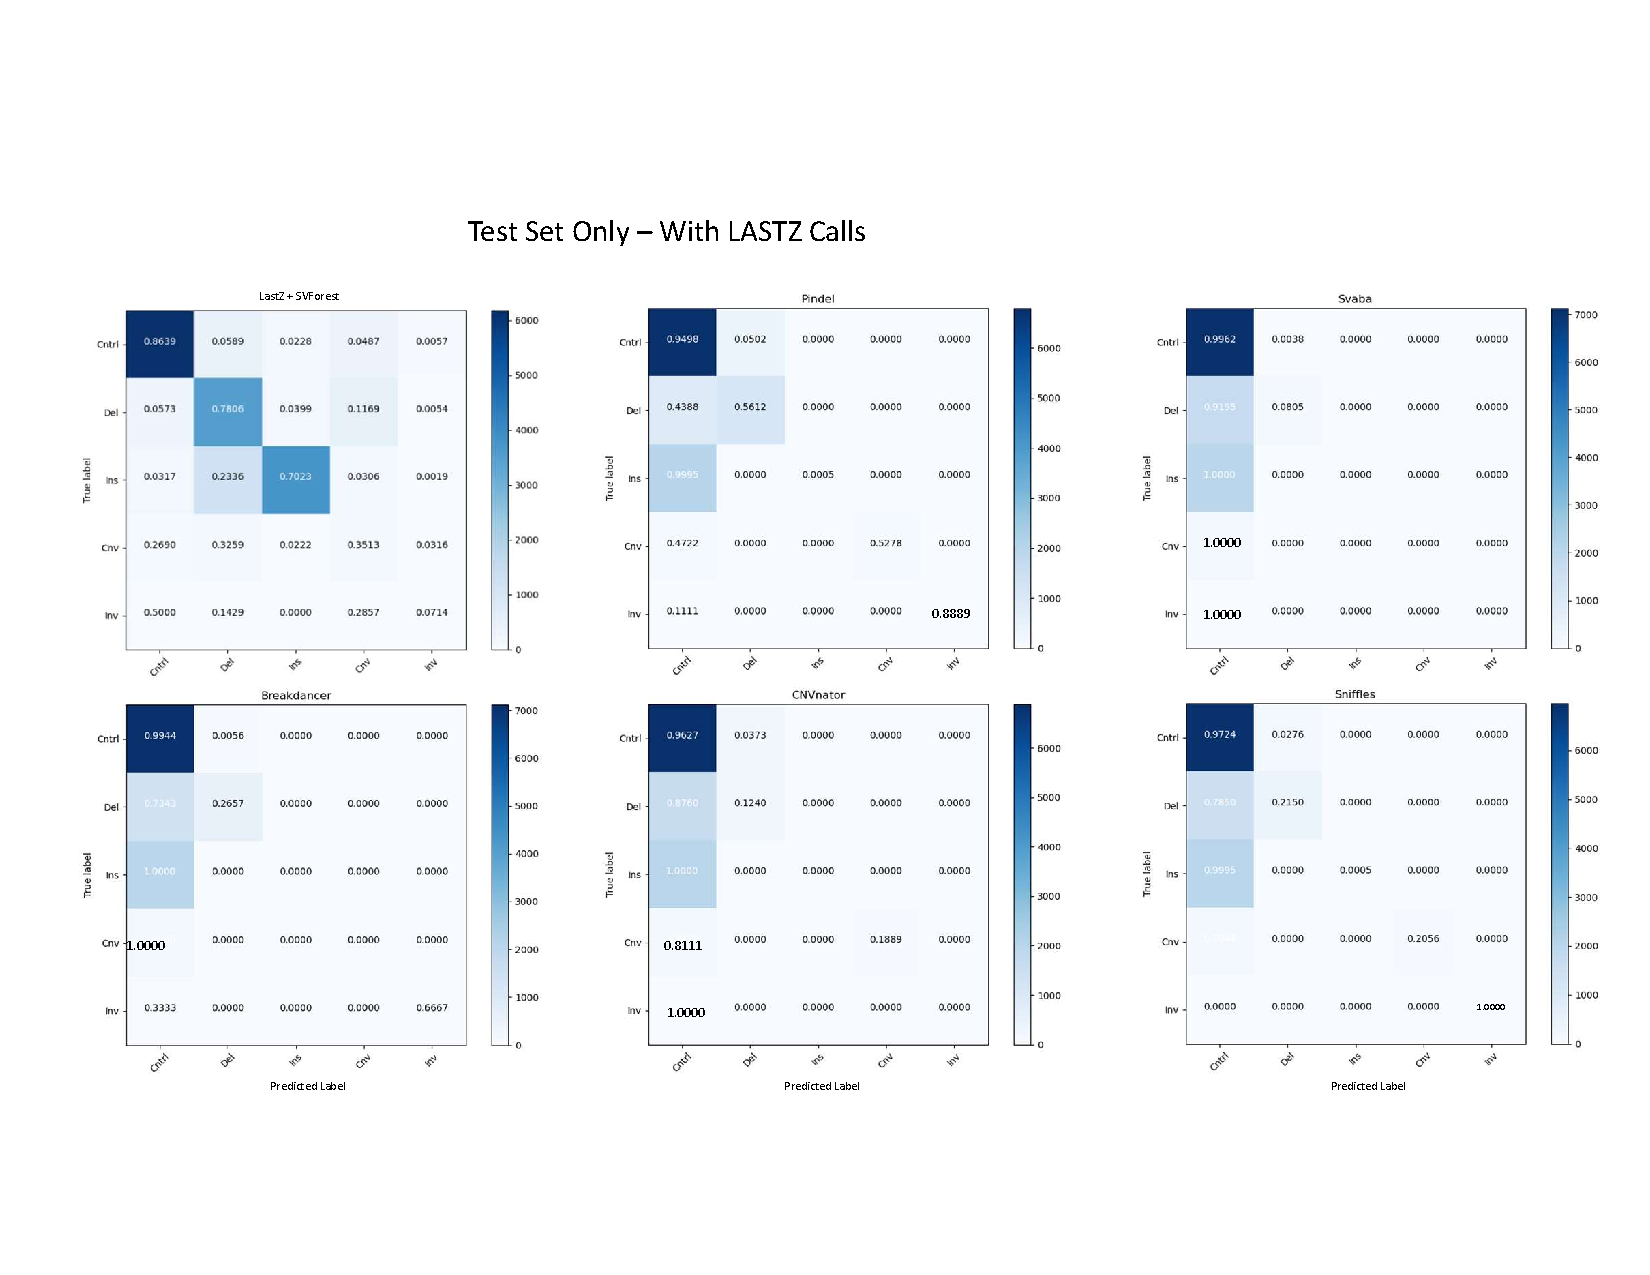
\includegraphics[width=\textwidth]{figures/ap3/caller_comparison.pdf}}
    \caption[SV calling benchmark.]{SV calling benchmark. Confusion matrices comparing multiple commonly-used callers to our LastZ calling combined with random forest genotyping approach. Values are reported as proportion of true labels (along the y-axis) that are included in a given intersection. Color indicates number of samples in a given intersection scaled to the largest number of samples in a class.}
    \label{fig:svbench}
\end{figure}


\begin{figure}
    \centering
    \makebox[\textwidth][c]{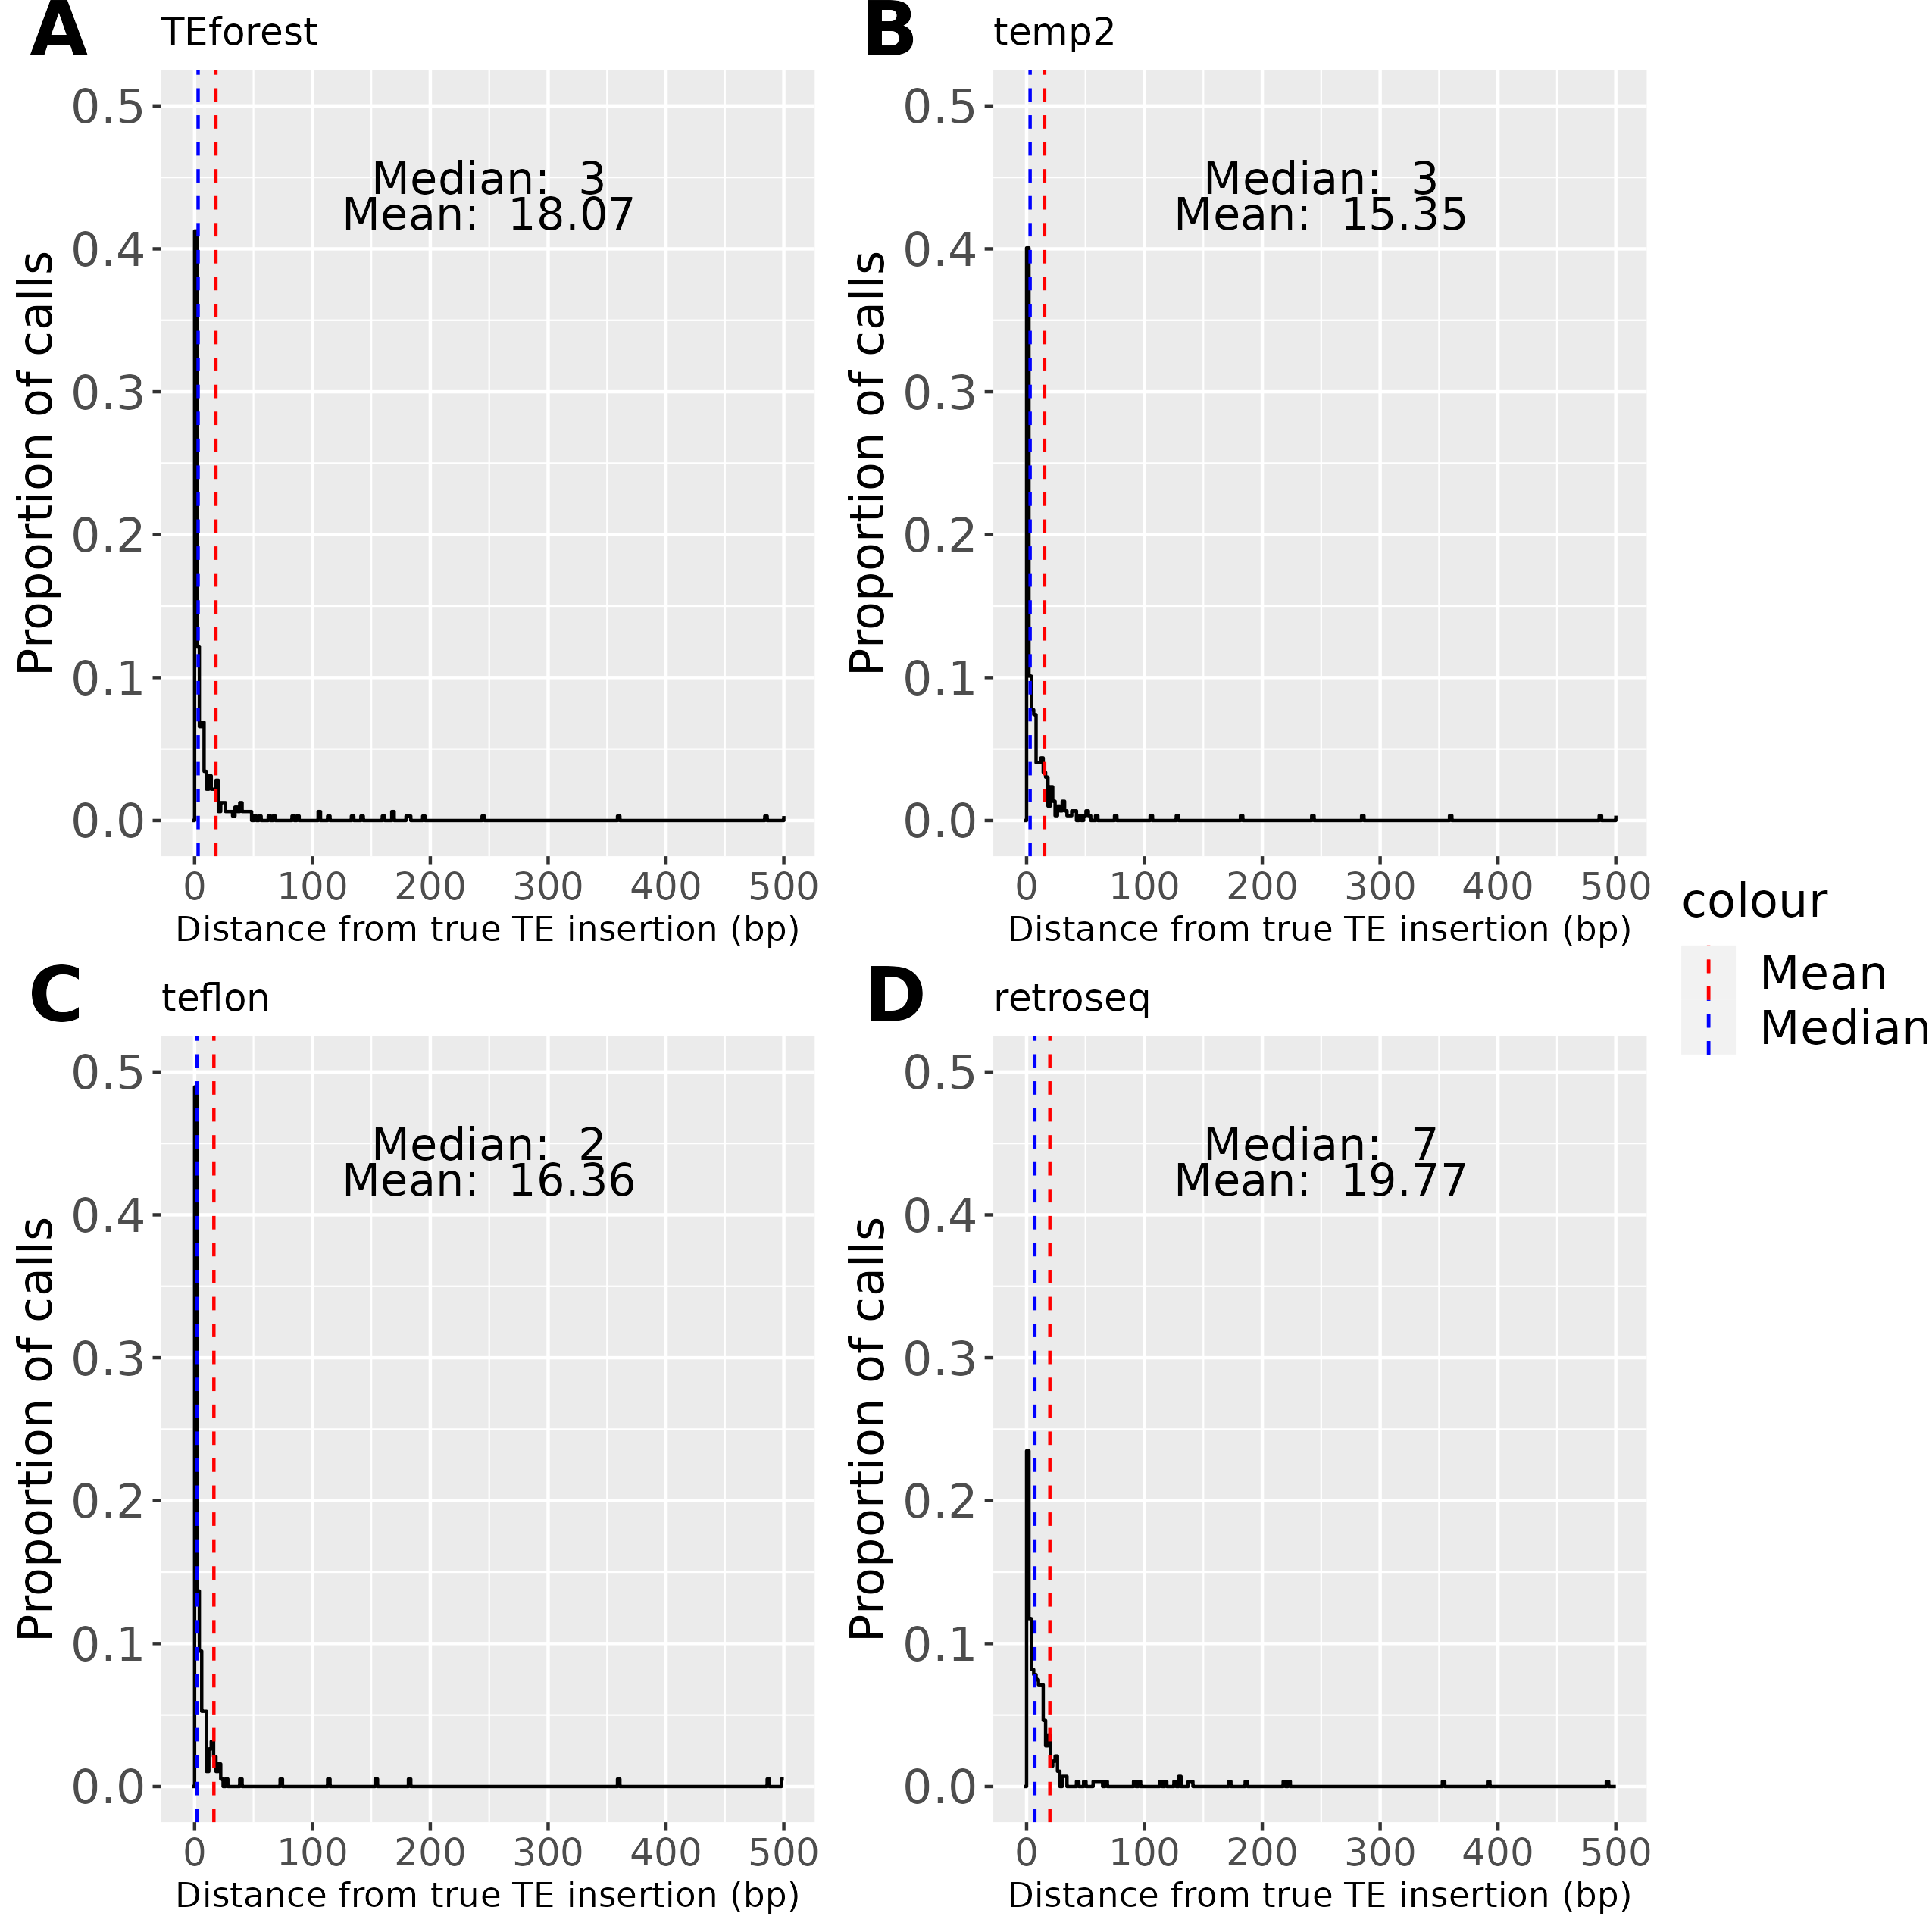
\includegraphics[width=\textwidth]{figures/ap3/breakpoints.png}}
    \caption[Accuracy of breakpoint identification for candidate TEs.]{Proportion of breakpoint calls versus their distance from the true TE insertion coordinate. Mean and median distance values are reported for each method and plotted as the red and blue dotted lines respectively. Values are reported for A) our method, dubbed "TEforest", B) temp2, C) teflon, and D) retroseq.}
    \label{fig:tebps}
\end{figure}

\begin{figure}
    \centering
    \makebox[\textwidth][c]{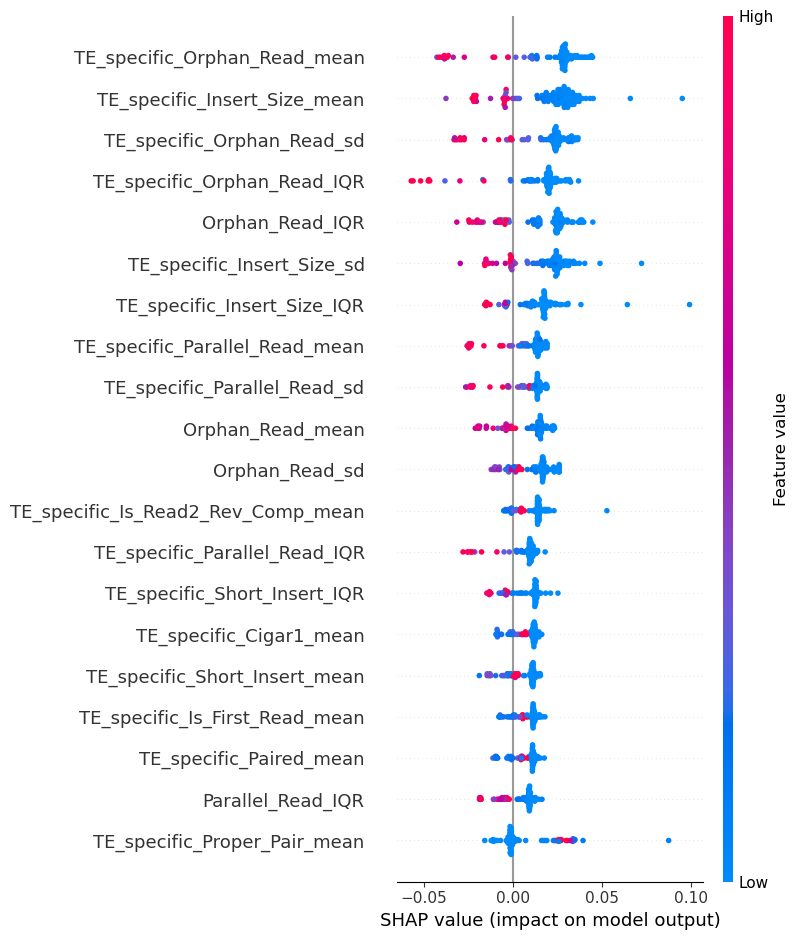
\includegraphics[width=\textwidth]{figures/ap3/shapley.png}}
    \caption[Shapley values for features used in TE genotyping prediction.]{Shapley values for features used in TE genotyping prediction. Plot generated with the shap R package, negative values indicate more strength in detecting TE presence, for example the mean orphan reads coverage (the top feature) has large amounts of predictions (individual points) with negative values that are also colored red, indicating high amount of importance for presence of TEs. }
    \label{fig:teshapley}
\end{figure}